\documentclass[10pt,draftclsnofoot,onecolumn,journal,compsoc]{IEEEtran}

\usepackage[margin=0.75in]{geometry}
\usepackage{graphicx}
\usepackage{caption}
\usepackage{hyperref}
\usepackage{enumerate}
\usepackage{pgfgantt}
\usepackage{tabu}
\usepackage[english]{babel}\usepackage[numbers]{natbib}
\usepackage{natbib}
\usepackage{vhistory}

\renewcommand{\bibsection}{}

\renewcommand{\linespread}{1.0}
\title{Prototype Big Data Archive in a Public Cloud}
\author{
  \IEEEauthorblockN{Group 56: Pathfinder of Big Data\\Zhi Jiang, Isaac T Chan, Zhaoheng Wang} \\
  \IEEEauthorblockA{CS 461: Senior Capstone Fall 2016 \\ Oregon State University}
}
\date{}

\IEEEtitleabstractindextext{
	\begin{abstract}
	OSU campuses generate data constantly from multiples sources, including computer labs, wireless usage, student devices, and many others. This quantity of data, also known as big data, can effectively represent all kinds of behaviors of students for information technology. Currently, the data is very difficult to manage because it is collected from multiple sources and is impossible to analyze. Therefore, this project requires the use of various technologies for support. There are nine pieces of technologies required:1) Methods to measure performance metrics of database functionality. 2) Methods of database security. 3) Methods of user interaction with the system. 4) The framework and storage of processing unprocessed data 5) The ingestion and parsing for unprocessed data.  6) The operation for formatted and cleaned data in data storage 7) The storage way for dealing with processed data. 8) The programming language for achieving database functionality. 9) The visualization tool use to display the data. For each piece, we will provide the best three technology options. Our goal for this paper is to analyze each technology option and determine the optimal technology that we will implement.
\end{abstract}
}

\begin{document}
% cover page    
    \maketitle
    \IEEEdisplaynontitleabstractindextext
    \IEEEpeerreviewmaketitle

    \newpage
% catalog    
    \tableofcontents
	\newpage

% revision history
	\begin{versionhistory}
  \vhEntry{1.0}{2017.02.06}{Zhi Jiang}{created revision history}
  \vhEntry{1.1}{2017.02.07}{Zhi Jiang}{modified the time line}
\end{versionhistory}
	\newpage     

% content    
	\section{Introduction}
	\subsection{Purpose}
    OSU campuses generate data constantly from multiples sources, including computer labs, wireless usage, student devices, and many others. This quantity of data, also known as big data, can effectively represent student behaviors for information technology. For example, analysis can be run to determine common student behaviors in order to allocate OSU resources to more often used utilities. Currently, the data is very difficult to manage because it is collected from multiple sources and is impossible to analyze. The data is neither stored in the same formats nor in the same locations, meaning it is inaccessible and useful information is unable to be extracted. The purpose of this project is to unify the data onto the consistent cloud platform of Amazon Web Services, which additionally provides utilities to manage and analyze.
    
    \subsection{Current Position}
    Currently, the functional part of the project is complete. We have a working database implementation in the Amazon Web Services public cloud, with appropriate storage, loading, and restricted access for sensitive data. By leveraging additional services in the AWS environment, we are able to provide rudimentary analysis, reporting, and visualization of data. From this position, we are able to present at Expo on the entire project, from beginning to end, including potential outcomes if the project were adopted by OSU. In the original project description, there were three deliverables listed. We have completed two of them: the database implementation and analysis/reporting/visualization. The third, a cost model, has yet to be complete. In order to provide an accurate cost model, we require an estimate for data amounts and are currently waiting for the estimate. This deliverable won't affect the project demonstration at Expo and is soley for the benefit of our client to decide on whether OSU will adopt our prototype.
	\newpage
	
	\section{Overall description}
	\subsection{Product perspective}
        In terms of perspective, our product is the most important part of a larger system. The larger system includes three parts, and which are importing data, managing data and analysing data, so main functionality of the product are used to import and manage data. The product is dependent on other parts of whole system because this product will relate to other services on AWS such as S3 as data storage and DynamoDB as database. On the other hand, we need to complete basic reporting and analysing function. Hence there should be data transmission between database and data analytics.
        
        \begin{figure}[h]
        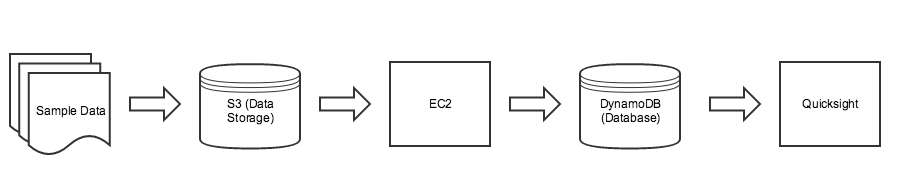
\includegraphics[width=18cm, height=4cm]{work_flow.png}
        \centering
        \caption{work flow of entire system}
        \end{figure}
        
	\subsection{Hardware Interface} 
       The database is built on public cloud so AWS platform will provide all aspects of the hardware supports. For example, high capacity solid state disks will used to store data items as a storage of product. And low-latency network connection can ensure maximum speed of accessing database.

	\subsection{Software interface}
        The AWS platform contains a variety of software provisioning for our product. On the one hand, developers can use proper programming language to implement functions of product base on via SDKs provided by AWS. On the other hand, the management console can help developer monitor all kinds of condition of database such as calculating throughput and cost. 
       
 	\subsection{Production function}
       The product will store different types of data such as log file, clickstream data in database. Besides, the product will provide enough space to hold vast amount of data, and it is able to build index and process data in batch. Furthermore, the database will implement some basic operations including inserting, deleting, updating and searching for data. Eventually, analysis technical will communicate to database, and then data will be accessed quickly by analysis technical while all of valuable data will be used to represent behaviors of students and staffs.

	\subsection{User characteristics}
        There is only one type of user that interact with our product: data analyzer. Staff who analyze the data can insert different types of data into database. Then, they could search the information base on the specific condition. After searching, data analyzer could do some management for the data such as sorting data. Finally, data analyzer could also extract the data from database and load it into a data analysis tool to do the analysis. 

	\subsection{Constraints}
        In implementation, there are minimal constraints placed on design. There are, however, certain aspects of development that we must keep in mind, including resource limits, implementation language, and development environment. The main aspect being that development on the AWS platform will cost our client money. AWS charges for computing time, temporary data storage, and database usage. Though it is unlikely that we will run into any upper budget limit, we need to have in mind the charges in order to eliminate resource waste. Amazon also offers a budget tool for our client to track our budget usage. It can also provide a forecast for future budget, so we can know in advance if we are approaching any limit. In terms of implementation language, AWS is flexible in the choice of coding language; we are free to choose any programming language that they support. Finally, our development will be done from our personal machines; as a cloud computing service, Amazon’s resources can be freely accessed by us wherever on any operating system.

	\subsection{Assumptions and dependencies}
        Because the nature of the project is to produce a prototype of a cloud-based big data archive, there is an assumption that our final product will be a competitive solution for OSU’s data analytics, compared to a locally-hosted solution. From this base-assumption, there are several dependencies to keep in mind, including scalability, future maintenance, and security.\\ 
        
        \noindent Our development will be done mostly with small test-sets of data, with student information anonymized before given to us. Therefore, a large concern is scalability - our solution must be able to work with potentially enormous data sets in a reasonable time. Database retrieval time is critical; the solution is almost useless if it takes an inappropriately long time to extract data from our implemented database. Additionally, database manipulation time, such as “joins” is an important factor when considering adopting the final product. Other metrics will be determined as we begin design implementation.
    
	\newpage
	
	\section{Specific requirements}
	\subsection{Functional requirements}
	\begin{itemize}
		\item The user can import any types of data into a NoSQl table in database from S3\\
        \textbf{Description:} In this function, the user should be able to import multiple data types into a NoSQL table in database through EC2 service\\
        \textbf{Sequence of operations:} 1) access EC2 service 2) run script to load file from S3 into local file 3) read data from local file 4) connect tbale in database 5) create new items to table\\
        \textbf{Test:} When importing different types of data in database, we need to check all of data should be imported in target table.\\
        
        \item The user can create a table for importing table\\
        \textbf{Description:} In this function, the user should be able to create a new table in NoSQL for storing data they want to import.\\
        \textbf{Sequence of operations:} 1) access EC2 service 2) run script to create a table in database 3) connect this table and import data in it\\
        \textbf{Test:} We can check wheather there exist a new table containing all data we have imported.\\
        
        \item The user can find information in database.\\
        \textbf{Description:} In this function, the user should be able to find information in database.\\ 
       \textbf{Sequence of operations:} 1) access the management console of database. 
        2) enter information which needs to be searched. 3) use searching function to search information in database 4) output related data items.\\ 
        \textbf{Test:} We can use unit testing to check correctness of results after we find a item.\\
        
        \item The user can do conditional find for information.\\
        \textbf{Description:} In this function, the user should be able to search information according some specific condition. For example, user can set some restrictions like they can only find data about senior students or engineering students.\\
        \textbf{Sequence of operations:} 1) access the management console of database. 2) enter information which needs to be search and set specific condition. 3) use search function to search information bases on condition. 4) output related data items.\\
        \textbf{Test:}: We can create specific unit testing according to finding condition. Then to use these unit testings to check correctness of results when we conditionally search an item.\\
        
        \item The user can aggregate data and then find specific result.\\
       	\textbf{Description:} In this functions, the user should be able to use aggregate methods to find some specific results such as average of GAP or the highest utilization ratio of certain printer on the campus.\\
        \textbf{Sequence of operations:} 1) access the management console of database. 2) enter result which needs to be aggregated. 3) use aggregation function to specific result. 4) output specific results.\\
        \textbf{Test:} We can use unit testing to check correctness of results after aggregate data. But we need to do some extra computing by ourselves for those specific results like average of GAP.\\
        
        \item The user can sort some specific data.\\
        \textbf{Description:} In this function, the user should be able to sort specified data. For example, user can sort amount of credits for all engineering students.\\
        \textbf{Sequence of operations:} 1) access the management console of database. 2) target a set of data which need to be sorted. 3) use sort function to sort a set of data. 4) output sorted list of data.\\
        \textbf{Test:} When database return sorted list, we can use unit testing to traversal the entire list and check correctness of relationship between adjacent items.
    \end{itemize}
	
	\subsection{Performance requirements}
        Performance metrics will be determined and assessed as we begin implementation. Currently there is no reliable basis of comparison for any performance metrics regarding database operations, such as data insertion, manipulation, and searching. A basis of performance comparison is subjective and may not fit our implementation exactly, thus are not defined at this point. Performance times for operations can be assessed by the client for acceptable runtimes and after client response, operating methods may be altered.
        
 	\subsection{Software system attributes}
 		\begin{itemize}
        \item{\textbf{Reliability:}}\\
        Compared to a locally hosted solution, a cloud platform offers additional benefits regarding reliability. When it comes to server maintenance, updates, and upgrades, downtime is a concern. Server downtime can interrupt analysis database access. Cloud platforms provide a reliable software system with minimal downtime\cite{AWS Rate}. There are agreements and certifications required by cloud providers\cite{Cloud} for acceptable amounts of downtime. As we implement our big data prototype with a cloud platform, reliability requirements are fulfilled by the cloud platform.\\
       
        \item{\textbf{Availability:}}\\
        Additionally, cloud platforms provide a method of access from anywhere, only requiring user credentials and an Internet connection. This is another benefit to the cloud solution.\\
   
        \item{\textbf{Security:}}\\
        Security is an important attribute. Our development will be using test-sets of user anonymized data, which protects us from liability and knowledge of specific users. Also, databases do have vulnerabilities, like any other software. We will consider prevention of malicious interactions, such as injection attacks. On the same note, if for any reason the database were to go down, we may want to have implemented a backup database. This will depend on the transfer time and quantity of data to store; if it is easily uploaded there is no reason to require a backup database.\\
     
        \item{\textbf{Maintainability:}}\\
        Future maintenance is another concern. Our implementation will be maintained by others of varying levels of expertise. Therefore, our product must have readable code and abundant, clear documentation.
    	\end{itemize}
	\newpage
	
	    \section{Schedule} 
        \begin{ganttchart}[vgrid, hgrid]{1}{22}
        \gantttitle{Fall}{4}
        \gantttitle{Winter}{10}
        \gantttitle{Spring}{8}\\
        
        \gantttitlelist{7, 8, 9, 10}{1}
        \gantttitlelist{1,...,10}{1}
        \gantttitlelist{1,...,8}{1}\\
        
        \ganttbar{Technology Review}{1}{1} \\
        \ganttbar{Design Plan}{2}{4} \\
        
        \ganttbar{Data storage Implementation}{5}{5} \\
        \ganttbar{Database table implementation}{5}{6}\\
        \ganttbar{Creating EC2}{7}{9}\\
        \ganttbar{Python script implementation}{9}{10}\\ 
        \ganttbar{Data visualization}{11}{12} \\
        
        \ganttbar{Test for functionality}{13}{15} \\
        \ganttbar{Performance Optimization}{14}{17}\\
        \ganttbar{Security Optimization}{17}{20}\\
        \ganttbar{Cost Comparison}{21}{22}
        \end{ganttchart}

	\newpage
	
% signature
	\thispagestyle{empty}
	\noindent\begin{tabular}{ll}
		\makebox[2.5in]{\hrulefill} & \makebox[2.5in]{\hrulefill}\\
		Client & Date\\[8ex]% adds space between the two sets of signatures
		\makebox[2.5in]{\hrulefill}\\
		Developer 1\\[8ex]
		\makebox[2.5in]{\hrulefill}\\
		Developer 2\\[8ex]
		\makebox[2.5in]{\hrulefill}\\
		Developer 3\\[8ex]
	\end{tabular}
\end{document}

